\documentclass[
	%parspace, % Add vertical space between paragraphs
	%noindent, % No indentation of first lines in each paragraph
	%nohyp, % No hyphenation of words
	%twoside, % Double sided format
	%draft, % Quicker draft compilation without rendering images
	%final, % Set final to hide todos
]{elteikthesis}[2024/04/10]

% The minted package is also supported for source highlighting
% See elteikthesis_minted.tex for example
%\usepackage[newfloat]{minted}
# Introduction of Container Evolution and Infrastructure Management via Code:
# Background: Start by outlining the history and evolution of container technologies. Highlight key milestones like the development of Docker, Kubernetes, and other container orchestration tools.
# Relevance of IaC: Discuss the rise of Infrastructure as Code (IaC) and how it has revolutionized managing and provisioning infrastructure through code, leading to more efficient and reproducible environments.
# Setup of a Comparative Case Study:
# Objective: Clearly define what you aim to compare in your case study and why. This could be comparing performance, scalability, or cost efficiency between different Kubernetes scaling strategies or between IaC tools.
# Methodology: Describe how you will implement these strategies, including the tools and technologies you will use. Make sure to detail any baseline configurations for fairness in comparison.
# Description of the Measurement Environment:
# Experimental Setup: Outline the hardware and software environments where the tests will be conducted. Include information on the Kubernetes clusters, the node specifications, and any other relevant infrastructure details.
# Metrics: Define what metrics you will measure (e.g., deployment time, resource usage, scaling efficiency) and how these metrics will be collected.
# Analysis of Results:
# Data Presentation: Use graphs, tables, and statistical analyses to present the collected data. Make sure your data visualizations are clear and effectively communicate the differences observed.
# Discussion: Interpret the results, discussing how they meet or do not meet your hypotheses or expectations. Analyze the implications of your findings in the context of existing literature.
# Further Improvements and Conclusion:
# Recommendations: Based on your findings, suggest improvements for the strategies or tools you tested. These could be optimizations for configurations or proposing areas for further development.
# Final Thoughts: Conclude your thesis by summarizing the key findings and their implications for the field. Reflect on the limitations of your study and suggest directions for future research.

% Document's metadata
\title{Auto-Scaling with Infrastructure-as-Code for Kubernetes-Driven Architectures} % title
\date{2024} % year of defense

% Author's metadata
\author{József Novák-Schwartz}
\degree{Mathematics BSc}

% Superivsor(s)' metadata
\supervisor{Győző Horváth} % internal supervisor's name
\affiliation{Associate Professor} % internal supervisor's affiliation
\extsupervisor{Zoltán Zvara} % external supervisor's name
\extaffiliation{Senior Developer} % external supervisor's affiliation

% University's metadata
\university{Eötvös Loránd University} % university's name
\faculty{Faculty of Informatics} % faculty's name
\department{Dept. of Software Technology and Methodology} % department's name
\city{Budapest} % city
\logo{elte_cimer_szines} % logo

% Add bibliography file
\addbibresource{elteikthesis.bib}

% The document
\begin{document}

% Set document language
%\documentlang{hungarian}
\documentlang{english}

% List of todos (not in the final document)
%\listoftodos[\todolabel]

% Title page (mandatory)
\maketitle
% Topic declaration page (mandatory) - can also be attached instead
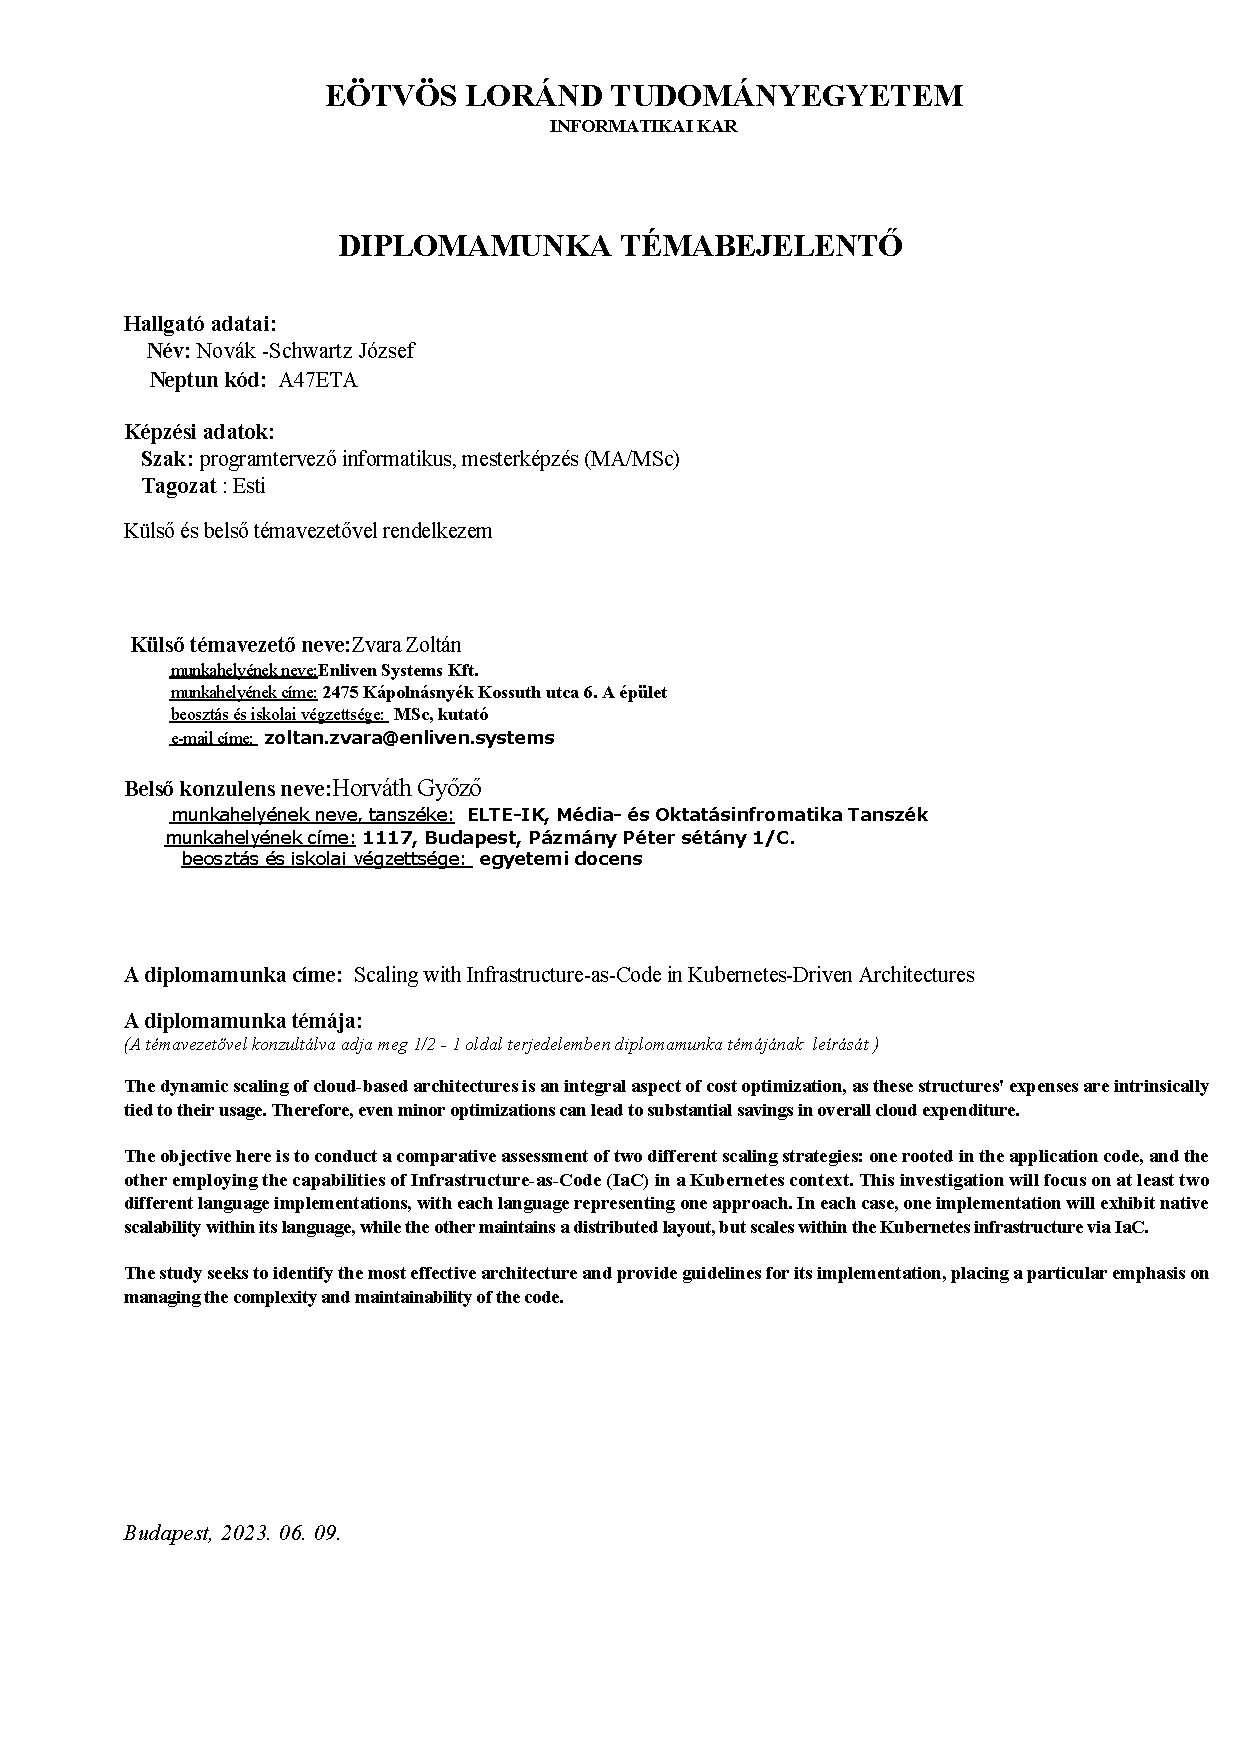
\includepdf{kerveny.pdf}

% Table of contents (mandatory)
\tableofcontents
\cleardoublepage

% Main content
\chapter{Introduction}
\label{ch:intro}

Software utilizes it's underlieing infrastructure. Preparing or setting up the infrastructure was mainly a manual process usually done by system administrators. They developed automations and applied system engineering principles which simplified the process. Infrastructure as Code means we can develop the software which provisions and sets up the hardware to be able to run our specified softwares. This way we can eliminate the so called "clickops" which used to mean the administrators operation done on user interfaces which were nit directly accessable by automation or they just did not developed automation for them yet. IaC enabled to track changes in git and the term Gitops means we were able to manage infrastructure similar way we manage our software code. We can test infrastructure changes on a branch then open a pullrequest and apply git development principles like 4 eye rule for the upcoming changes.
My research is based on this: since we can manipulate infrastructure as easy and fast as any code, we might change our perspective in some programming cases. Scaling up and down usually involved some internal logic in the code which we can now outsource to our infrastructure code.


\cleardoublepage


% Acknowledgements (optional) - in case your thesis received funding or would like to express special thanks to someone
\chapter*{\acklabel}
\addcontentsline{toc}{chapter}{\acklabel}
In case your thesis received financial support from a project or the university, it is usually required to indicate the proper attribution in the thesis itself. Special thanks can also be expressed towards teachers, fellow students and colleagues who helped you in the process of creating your thesis.

% Appendices (optional) - useful for detailed information in long tables, many and/or large figures, etc.
\appendix

% Bibliography (mandatory)
\phantomsection
\addcontentsline{toc}{chapter}{\biblabel}
\printbibliography[title=\biblabel]
\cleardoublepage

% List of figures (optional) - useful over 3-5 figures
\phantomsection
\addcontentsline{toc}{chapter}{\lstfigurelabel}
\listoffigures
\cleardoublepage

% List of tables (optional) - useful over 3-5 tables
\phantomsection
\addcontentsline{toc}{chapter}{\lsttablelabel}
\listoftables
\cleardoublepage

% List of algorithms (optional) - useful over 3-5 algorithms
\phantomsection
\addcontentsline{toc}{chapter}{\lstalgorithmlabel}
\listofalgorithms
\cleardoublepage

% List of codes (optional) - useful over 3-5 code samples
\phantomsection
\addcontentsline{toc}{chapter}{\lstcodelabel}
\lstlistoflistings
\cleardoublepage

% List of symbols (optional)
%\printnomenclature

\end{document}
